\documentclass{elsarticle}
\usepackage{amssymb}
\usepackage{amsmath}
\usepackage{bigdelim}
\usepackage{multirow}
\usepackage{hyperref}
\usepackage{graphics}
\usepackage{algorithm}
\usepackage{algorithmic}
%\usepackage{algorithmicx}
\journal{Expert System with Applications}

\newtheorem{definition}{Definition}


\begin{document}

\begin{frontmatter}
\title{A Complex Network Model of Knowledge Collaboration in Virtual Community: Based on Wiki Community
}
\author[buaa]{Jun Wang}
\ead{king.wang@buaa.edu.cn}

\author[buaa]{Yunpeng Wu}
\ead{yunpeng.wu@sem.buaa.edu.cn}

\author[buaa]{Xin Jin}
\ead{sssss}

\address[buaa]{School of Economics and Management, Beihang University, 
Beijing 100083, P.R. China}

\begin{abstract}
  
\end{abstract}

\begin{keyword}
Wikipedia, Knowledge collaboration network, Scale-free structure,
Small-world effect, Topic Approximation, scale ratio
  
\end{keyword}
\end{frontmatter}

\section{Introduction}
\label{sec:introduction}

In the past few years, complex network is being infiltrated into sociology, mathematics, life sciences, engineering and many other different areas, the scientific understanding to the quantitative and qualitative characteristics of complex network has become a challenging and important issues of scientific research in the Internet era, and even referred to as "the network's new science"[1-2]. Social networks, which are an important examples of complex networks, have many similar properties with complex networks [3]. For example, the short length of the average shortest-path distance, the high value of the clustering coefficient and the scale-free distribution of connectivity are some of the common properties of those networks [4-6].In other words, there are many similar conclusions among them, such as “small worlds” effect[7],scale-free[8], power law[9] and so on. 

In recent years, bipartite networks have attracted more and more people's attention [10-13]. Factuallyt, many real-world networks are naturally bipartite, such as the actors-films network [11], the Scientist Co-authorship Collaboration network [12-13], the knowledge-cooperation network and so on.

Wiki system as the typical knowledge-cooperation newtork and virtual practice community has become more and more popular in knowledge management system field. It is an important approach to publish on-line information and a different way to collaborate. They can be characterized as ‘‘ultra-lightweight’’ content management systems [14]. Wiki is a method for knowledge cooperation and refers to a collaborative hyper medium that allows for continuous communication within a research team and the constant evolution of content [15].Wikis are used for a diversified number of applications: some as databases for research and writing, as personal information manager, as collaborative tool between teams to create and maintain documents that need to be updated frequently, etc.

Wiki network is different from other social networks on the WWW,such as Sina Blog. The collaboration in Blog is non-themed or variable- themed. However, for the same theme, the collaboration in wiki is expanding denotedly and connotedly. It will talk about a topic with a very full depth [16].

In the current studies, complex network has shown a lot of valuable properties [7-13,17]. This paper focuses on two aspects: the wiki one-dimensional network, ties connected between users; the bipartite network, the ties connected users and topics. Through an empirical study of en-Wikipedia network’s data which is from January 2004 to January 2008, we discover that many properties of wiki network are similar with other networks. 

The rest of the paper is organized as follows. In section II, we
introduce the complex social network mould wiki-based knowledge
collaboration. The empirical analysis of the one-dimensional
properties is presented in section III. On the meanwhile, section IV
proposes the pilot study of the wiki bipartite network, namely, the
relationship between network properties and scale. Section V is
devoted to our conclusions and discussions.

\section{The network structure of Wiki-based knowledge collaboration}
\label{sec:netw-struct-wiki}

Wikipedia is a typical Knowledge collaboration- oriented virtual community, in which the group who has the same interest in the same topic can communicate and interact with each other through topic pages to participate in the knowledge collaboration activities. Wikipedia can be depicted as an open content encyclopedia,the open materials of which allow unrestricted access to any third party to copy, modify, thus, it  provides great convenience for people from various sectors. On the meantime, the users can increase their knowledge and enrich themselves. As of April 25, 2009, according to Wikipedia statistics (Wiki Stats Statistics) [18], the English version has 16,550,111 entries, user groups have been 9,505,160.Over a period of time, there will be a certain number of user groups to participate in the discussion of a topic.

As to the characteristics of Wikipedia knowledge collaboration network, the authors of this paper build a collaborative Wiki-based knowledge network model, as shown in Figure 1. There are also two types of ties: C and A: C is the collaboration among users, shown as white lines in Fig.1, while the A express the affiliation between T and U, shown as dark color lines in Fig.1. The collaboration relationship among C ties comes into being through participating in the A ties discussions.  

\begin{figure}[h]
  \centering
  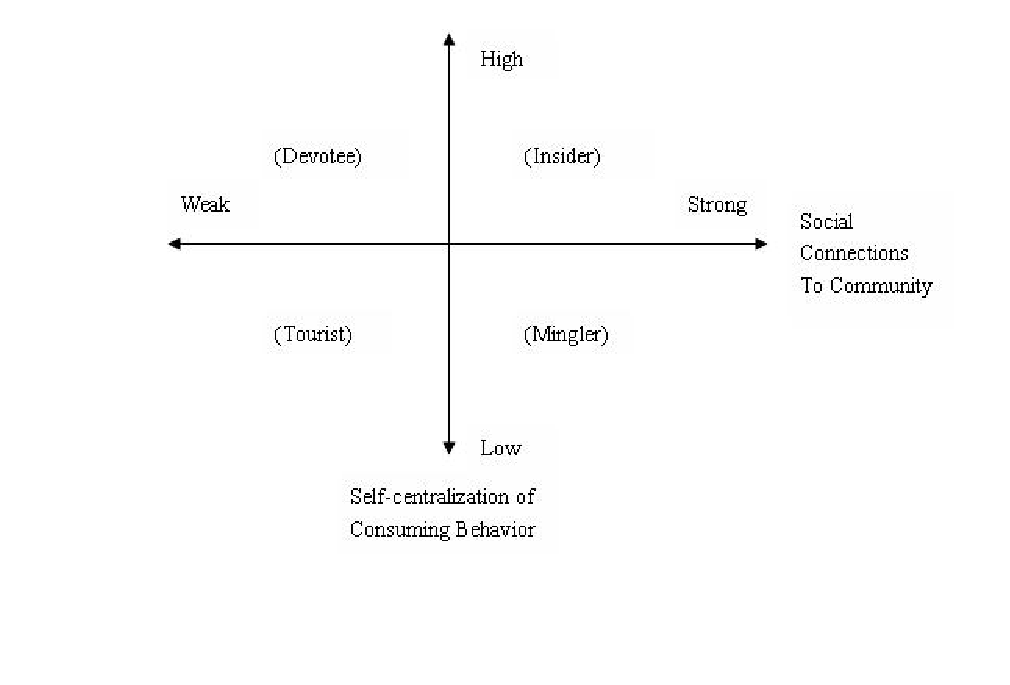
\includegraphics{01}
  \caption{The Two-dimensional, Wiki-based Knowledge Collaboration Network Mould}
\end{figure}

From the network model in figure 1, it is easily found that this model
includes two complex networks: one-dimensional networks of
single-layer and bipartite two-dimensional networks. 

In the single-layer networks, all the users in the same Topic collaboration process builds Undirected and Unweighted Complete Sub-graph (UUCSG), shown as [u1-u2] [u3-u6] [u6-u10] [u9-u12] in Fig.1.The entire single-layer network is composed of n UUCSGs, in which N represents the number of Topics. The whole network can be expressed as an adjacency matrix “Bu”.

 the bipartite networks, the UUCSG is constructed by all the UUCSGs in
 the single-layer networks and the topics which the UUCSG belong
 to. The number of nodes is equal to the numbers of the User
 nodes. Therefore, the bipartite networks can be described as an
 adjacency matrix “Bt”. The ratio between Users and Topics exists in
 the bipartite networks, which is called scale ratio and can be
 described as
 \begin{math}
 W = N_{user}/N_{topic}   
 \end{math}
This model does not clearly define the direction of the relationship, thus, the model belongs to Undirected and Unweighted Complete Sub-graph. However, such network model vividly displays virtual communities of practice networks which aims for knowledge collaboration and innovation, such as Wikipedia.



\begin{align*}
       a=
       \left\begin{matrix} 
 &u_1 & u_2 \\  
 u_1\ldelim[{2}{0.1cm}&1&0\rdelim]{2}{0.1cm}\\
 u_2 &0&1\\
\end{matrix}
& \qquad \qquad \begin{vmatrix} 1 & 2 & 3 \\ 3 & 4 & 5 \end{vmatrix}
\end{align*}


\bibliographystyle{elsarticle-num}
\bibliography{../../bibtex/elsevier,../../bibtex/emerald,../../bibtex/chinese,../../bibtex/jstor,../../bibtex/citeseer,../../bibtex/acm,../../bibtex/wiley,../../bibtex/book,../../bibtex/thesis,../../bibtex/ebsco,../../bibtex/old,../../bibtex/ieee,../../bibtex/internet,../../bibtex/ssrn,../../bibtex/apa,../../bibtex/blackwell,../../bibtex/sage,../../bibtex/springer,../../bibtex/MESharp,../../bibtex/taylor}
\end{document}
